\documentclass[tikz,border=2pt]{standalone}
\usepackage{amsmath,amssymb}
\usetikzlibrary{arrows.meta,positioning,fit,calc,backgrounds}

\definecolor{cTeacher}{HTML}{6C5CE7}
\definecolor{cSlow}{HTML}{2878B5}
\definecolor{cFast}{HTML}{E67E22}
\definecolor{cNom}{HTML}{2E8B57}
\definecolor{cRes}{HTML}{C0392B}
\definecolor{cInk}{HTML}{263238}

\tikzset{
  flow/.style={-{Latex[length=2.2mm]},line width=0.75pt,draw=cInk},
  data/.style={rounded corners=2pt,draw=cInk!65,fill=gray!7,line width=0.65pt,
               align=center,minimum height=8mm,text width=22mm,font=\sffamily\scriptsize},
  teacher/.style={rounded corners=3pt,draw=cTeacher,fill=cTeacher!10,line width=1.1pt,
                  align=center,minimum height=18mm,text width=31mm,font=\sffamily\small\bfseries},
  query/.style={rounded corners=2pt,draw=cTeacher!80,fill=white,line width=0.8pt,
                align=center,minimum height=9mm,text width=28mm,font=\sffamily\scriptsize},
  target/.style={rounded corners=2pt,line width=0.9pt,align=center,minimum height=9mm,
                 text width=27mm,font=\sffamily\scriptsize\bfseries},
  student/.style={rounded corners=3pt,line width=1.1pt,align=center,minimum height=17mm,
                  text width=30mm,font=\sffamily\small\bfseries},
  slowbox/.style={rounded corners=3pt,draw=cSlow,fill=cSlow!9,line width=1pt,align=center,
                  minimum height=17mm,text width=30mm,font=\sffamily\scriptsize\bfseries},
  bad/.style={rounded corners=2pt,draw=cInk!45,fill=gray!8,line width=0.7pt,align=center,
              text width=33mm,font=\sffamily\tiny},
  good/.style={rounded corners=2pt,draw=cFast,fill=cFast!12,line width=0.9pt,align=center,
               text width=33mm,font=\sffamily\tiny\bfseries},
  note/.style={font=\sffamily\tiny,align=center,text=cInk!75}
}

\begin{document}
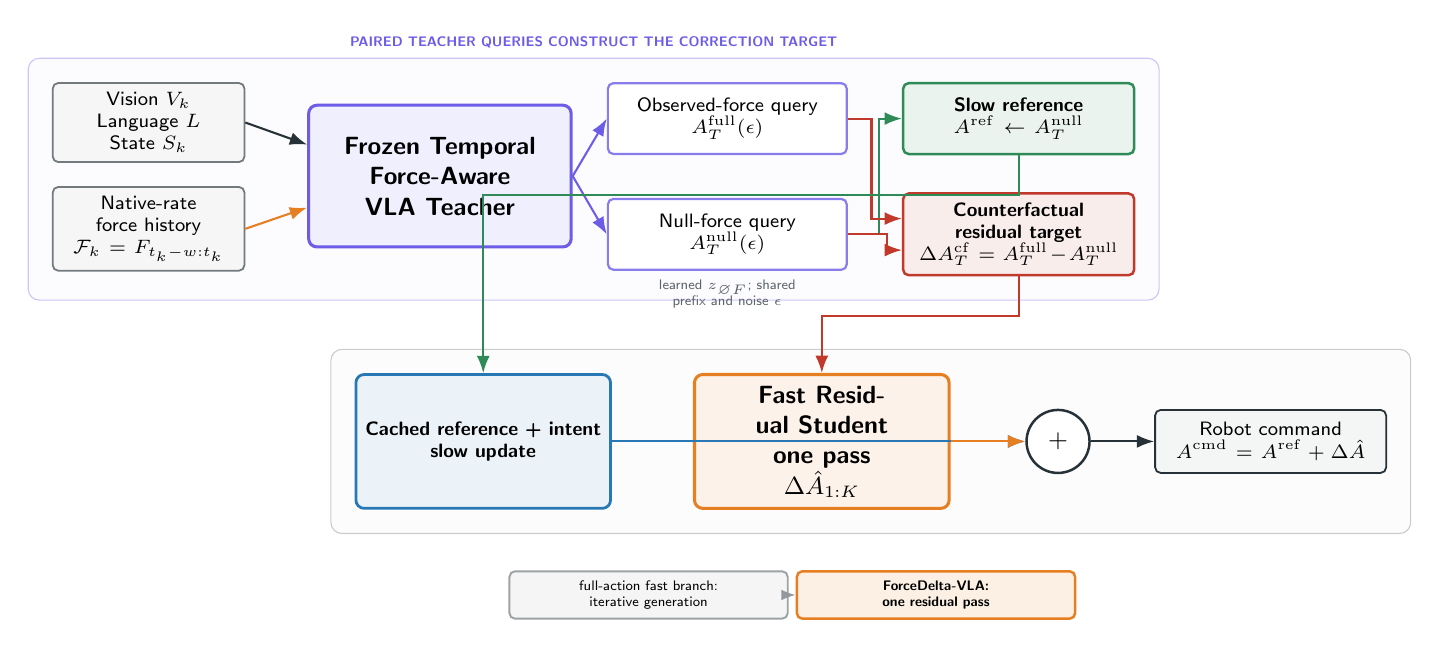
\begin{tikzpicture}
  % Top: paired target construction.
  \node[data] (vls) at (0,2.0) {Vision $V_k$\\Language $L$\\State $S_k$};
  \node[data] (force) at (0,0.65) {Native-rate force history\\$\mathcal{F}_k=F_{t_k-w:t_k}$};
  \node[teacher] (teach) at (3.7,1.32) {Frozen Temporal\\Force-Aware\\VLA Teacher};
  \draw[flow] (vls.east) -- ([yshift=4mm]teach.west);
  \draw[flow,draw=cFast] (force.east) -- ([yshift=-4mm]teach.west);

  \node[query] (full) at (7.35,2.05) {Observed-force query\\$A_T^{\mathrm{full}}(\epsilon)$};
  \node[query] (null) at (7.35,0.58) {Null-force query\\$A_T^{\mathrm{null}}(\epsilon)$};
  \draw[flow,draw=cTeacher] (teach.east) -- (full.west);
  \draw[flow,draw=cTeacher] (teach.east) -- (null.west);
  \node[note,text width=31mm] at (7.35,-0.18)
    {learned $z_{\varnothing F}$; shared prefix and noise $\epsilon$};

  \node[target,draw=cNom,fill=cNom!10] (nom) at (11.05,2.05)
    {Slow reference\\$A^{\mathrm{ref}}\!\leftarrow\!A_T^{\mathrm{null}}$};
  \node[target,draw=cRes,fill=cRes!9] (res) at (11.05,0.58)
    {Counterfactual residual target\\$\Delta A_T^{\mathrm{cf}}=A_T^{\mathrm{full}}\!-\!A_T^{\mathrm{null}}$};
  \draw[flow,draw=cNom] (null.east) -- ++(4mm,0) |- (nom.west);
  \draw[flow,draw=cRes] (full.east) -- ++(3mm,0) |- ([yshift=2mm]res.west);
  \draw[flow,draw=cRes] (null.east) -- ++(5mm,0) |- ([yshift=-2mm]res.west);

  % Bottom: asynchronous deployment.
  \node[slowbox] (slow) at (4.25,-2.05)
    {Cached reference + intent\\slow update};
  \node[student,draw=cFast,fill=cFast!10] (fast) at (8.55,-2.05)
    {Fast Residual Student\\one pass\\$\Delta\hat{A}_{1:K}$};
  \node[circle,draw=cInk,fill=white,line width=0.9pt,minimum size=8mm,
        font=\sffamily\small\bfseries] (sum) at (11.55,-2.05) {$+$};
  \node[data,text width=27mm,draw=cInk,fill=cInk!5] (cmd) at (14.25,-2.05)
    {Robot command\\$A^{\mathrm{cmd}}=A^{\mathrm{ref}}+\Delta\hat{A}$};

  \draw[flow,draw=cNom] (nom.south) -- ++(0,-5mm) -| (slow.north);
  \draw[flow,draw=cRes] (res.south) -- ++(0,-5mm) -| (fast.north);
  \draw[flow,draw=cSlow] (slow.east) -- (sum.west);
  \draw[flow,draw=cFast] (fast.east) -- (sum.west);
  \draw[flow] (sum.east) -- (cmd.west);

  \node[bad] (before) at (6.35,-4.0)
    {full-action fast branch:\\iterative generation};
  \node[good] (after) at (10.0,-4.0)
    {ForceDelta-VLA:\\one residual pass};
  \draw[dashed,line width=0.6pt,draw=cInk!50,-{Latex[length=1.8mm]}]
    (before.east) -- (after.west);

  \begin{scope}[on background layer]
    \node[rounded corners=4pt,draw=cTeacher!35,fill=cTeacher!2,inner sep=3mm,
          fit=(vls)(force)(teach)(full)(null)(nom)(res),
          label={[font=\sffamily\tiny\bfseries,text=cTeacher]above:PAIRED TEACHER QUERIES CONSTRUCT THE CORRECTION TARGET}] {};
    \node[rounded corners=4pt,draw=cInk!25,fill=gray!2,inner sep=3mm,
          fit=(slow)(fast)(sum)(cmd)] {};
  \end{scope}
\end{tikzpicture}
\end{document}
